\begin{figure}[H]
	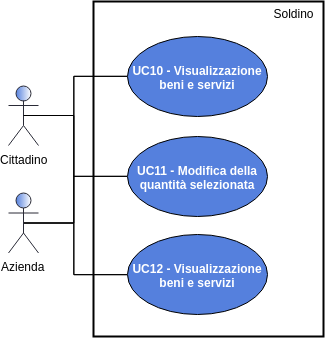
\includegraphics[width=6cm]{res/images/benieservizi.png}
	\centering
	\caption{Beni e servizi}
\end{figure}
\subsubsection{UC10 - Visualizzazione beni e servizi}

 \begin{itemize}
 	\item \textbf{Attori Primari}: cittadino, azienda;
 	\item \textbf{Descrizione}: l'utente visualizza una lista contenente tutti i beni/servizi in vendita sulla piattaforma. Per ogni prodotto vengono visualizzate le seguenti informazioni:
 	\begin{itemize}
 		\item nome;
 		\item prezzo lordo\glosp (in Cubit\glo);
 		\item descrizione;
 		\item quantità di prodotto selezionata.
 	\end{itemize}
 	
 	\item \textbf{Scenario principale}: l'utente si trova all'interno della pagina per la ricerca dei prodotti e sta visualizzando dei beni/servizi;	
 	\item \textbf{Precondizione}: l'utente accede alla pagina del sito dedicata alla visualizzazione dei prodotti in vendita;
 	\item \textbf{Postcondizione}: l'utente visualizza le informazioni relative ai prodotti, con le eventuali operazioni disponibili su ognuno di essi.
 \end{itemize}

 \subsubsection{UC11 - Modifica della quantità selezionata}
 \begin{itemize}
 	\item \textbf{Attori Primari}: cittadino, azienda;
 	\item \textbf{Descrizione}: l'utente può modificare la quantità selezionata di un prodotto utilizzando il campo apposito;
 	\item \textbf{Scenario principale}: l'utente modifica la quantità di un prodotto utilizzando l'apposito campo;
 	\item \textbf{Precondizione}: l'utente sta visualizzando un prodotto ed intende modificarne la quantità selezionata;
 	\item \textbf{Postcondizione}: la quantità del prodotto è stata aggiornata al nuovo valore richiesto.
 \end{itemize}

 \subsubsection{UC12 - Ricerca di beni/servizi}
\begin{itemize}
	\item \textbf{Attori Primari}: cittadino, azienda;
	\item \textbf{Descrizione}: L'utente usare una barra di ricerca per cercare i prodotti richiesti. La barra di ricerca filtra i prodotti usando una parola o una frase chiave;
	\item \textbf{Scenario principale}: l'utente porta il cursore sulla barra di ricerca e digita una parola chiave;
	\item \textbf{Precondizione}: l'utente sta visualizzando i prodotti necessita di fare una ricerca specifica;
	\item \textbf{Postcondizione}: la ricerca è avvenuta e restituisce per risultato l'insieme di oggetti richiesti.
\end{itemize}